% Some LaTeX commands I define for my own nomenclature.
% If you have to, it's better to change nomenclature once here than in a 
% million places throughout your thesis!
\newcommand{\package}[1]{\textbf{#1}} % package names in bold text
\newcommand{\cmmd}[1]{\textbackslash\texttt{#1}} % command name in tt font 


%======================================================================
\chapter{MAFOSS}
\label{chap:MAFOSS}
%======================================================================


\section{Introduction}
\label{sec:introductionMAFOSS}
This chapter presents a new multi-agent framework using open-source software (MAFOSS). The proposed framework is a modular and cost-effective open-source hardware and software platform that is intended to help develop multi-agent systems for research and education.  Numerous multi-agent platforms have been developed in the literature to date that are used in various robotic applications, such as surveillance, target localization, cooperative estimation, among others. However, most of them are either tailored towards particular applications or driven by expensive software and hardware. The proposed MAFOSS system is developed for robotic applications, where a team of mobile agents (robots) is deployed to achieve a common goal. The software architecture of the current framework mostly relies on robot operating system (ROS). Regardless of internal hardware and/or software architecture, appropriate actions can be applied to actuators of an individual or a team of mobile agents for controlling their motions. A few case studies have been conducted to evaluate the performance of MAFOSS.


The development of multi-agent systems has been of crucial importance in modern autonomous agent-based applications, such as area coverage~\cite{Cortes2004,Lekien2009,MiNgBoSp2014-j1}, perimeter surveillance and environment monitoring~\cite{Pimenta2013,Zhang2013,Rossi2016},  cooperative estimation and formation control~\cite{Spinello2014,Marshall2004,Ge2017,Li2017}, indoor navigation~\cite{GuMi2008-j1,KnHeMi2017-c1} using mobile robots, among others. Typical problems in such applications are usually solved using an array of networked mobile agents operating collectively. Recently, the implementation of various algorithms has been restricted to a fleet of homogeneous robots at high monetary cost. The purpose of this research is to lower the costs of entry due to the selected robot platform by providing an easily accessible framework for heterogeneous robots that can be implemented both expediently and efficiently. Note that the terms robot and agent will be used interchangeably from now on.  While the performance of the most promising multi-agent control algorithms proposed in the literature is evaluated using computer simulations only, a few multi-agent control algorithms have been validated using experiments that fit for particular implementation platforms (\textit{i.e.,} use of specific robots, for example). See the work performed by authors in~\cite{Marshall2004,MiKn2018-j1,MiKnHe2018-j1}, for instance. Therefore, this paper aims to develop an open hardware/software architecture, MAFOSS, to implement multi-agent control algorithms. Two case studies have been implemented using MAFOSS. Some of the major advantages of the MAFOSS include its scalability, low cost, robustness, and open source nature. These qualities enable users to develop algorithms on a larger scale than was previously possible. 
%
The open source environment brings a wide range of support whilst maintaining a fast moving and non-proprietary code base. There are many packages in ROS that allow a user to interface sensors, actuators, and other hardware directly into their system with minimal development required. As such, it is an excellent tool for anyone looking to expand or help standardize their implementation of different algorithms in the fields of cooperative estimation and navigation. 



\section{Overall MAFOSS Architecture}
\label{sec:overallArchitecture}
The overall architecture of the proposed MAFOSS is shown in  Fig.~\ref{fig:MAFOSS-OverallArchitecture}. %
%
\begin{figure}
  \centering
  \fcolorbox{blue}{gray!5}{
    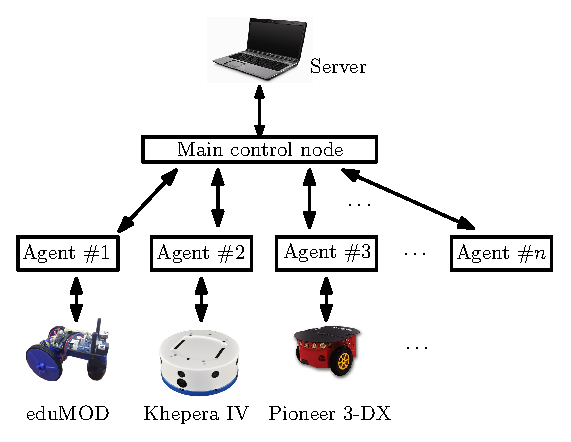
\includegraphics[width=0.45\textwidth]{figs/ipe/networkingOutline.eps}
  }
    \caption{Overall architecture of MAFOSS.}
    \label{fig:MAFOSS-OverallArchitecture}
\end{figure}
%
Therein, $n$ (mobile) agents and the main control node are connected through a local or wide area network used in the proposed framework. After the network has been configured, a multi-agent algorithm can be implemented in the central node. Using this algorithm, the actuator commands determined by the central node are sent to all agents for appropriate actions. The agents collect the measurements and pass relevant data back to the central node as well as prepare to receive new data. All the agent platforms are running ROS, an open source robotics operating system. The client software installed in the central node depends on a particular application within a multi-agent systems. For example, the authors of this paper have documented two case studies where MATLAB's Robot System Toolbox\footnote{https://www.mathworks.com/products/robotics.html} was used as the client software. Note that MATLAB is not open-source, however the decision to use MATLAB was done to save time in the implementation process.  

As a proof of concept, let us consider an area coverage problem~\cite{MiKn2018-j1,MiFaSp2017-j1,MiPaFaSp2017-j1,MiNgBoSp2015-j1}, where a group of mobile autonomous agents are deployed in an area of interest. The problem is to deploy a group of mobile agents such that the coverage metric is maximized. In this case, the central node of the proposed MAFOSS architecture is assigned to implement the area coverage algorithm. For that, appropriate actuator commands for each mobile agent are dispatched at a regular time intervals. The details on how these area coverage algorithms work can be sought in~\cite{MiKn2018-j1,MiFaSp2017-j1,MiPaFaSp2017-j1,MiNgBoSp2015-j1}.  The next section illustrates the software architecture of the MAFOSS that can be used to implement a set of algorithms that use autonomous agents for solving problems of multi-agent systems.
  

%================================================================================================
%================================================================================================
\section{Software Architecture}
\label{sec:softwareArch}
Fig~\ref{fig:MafossSoftwareArchitecture} shows the higher-level software architecture of the proposed MAFOSS. %
%
\begin{figure}
  \centering
              \begin{tikzpicture}
                \tikzstyle{every node} = [font =\small]
                % \tikzstyle{block} = [draw, fill=blue!20, rectangle, 
                % minimum height=3em, minimum width=6em]
                \tikzstyle{block} = [draw, fill=blue!20, rectangle, rounded corners]      
                \tikzstyle{pinstyle} = [pin edge={to-,thin,black}]
                % 
                % 
                \node [block,text width=0.45\textwidth] (userApplication) { \centering \ul{Higher--level application program running at central node}\\
                  \begin{center}
                    $\bullet$~Application program \qquad$\bullet$ ROS logging
                  \end{center}  
                };
                \node[block, text width=0.45\textwidth, below of =userApplication, node distance=3.0cm](ROS){
                  \centering 
                  \ul{Robot Operating System (ROS) }\\
                  \begin{center}
                    $\bullet$~ROS agents \qquad$\bullet$ ROS networking
                  \end{center}
                  };                    
                \node[block, text width=0.45\textwidth, below of =ROS, node distance=3.0cm](controlAPI){
                  \centering 
                  \ul{Lower--level APIs running at high bandwidth}\\
                  \begin{center}
                    $\bullet$~Robot control libraries, such as \emph{librobotcontrol}, \emph{ROS aria}, and \emph{libkhepra}
                  \end{center}
                };
                \node[block, text width=0.45\textwidth, below of =controlAPI, node distance=3.0cm](agents){
                  \centering 
                  $\text{Agent}~\#1~\ldots~\text{Agent}~\#n$ running lower--level actuator commands at high bandwidth
                  };                                 
                % \node[block, text width=1.5cm, right of =inSignalConditioning, node distance=3.5cm](ADC){\emph{BBBlue's 12-bit ADC}};                
                % Draw arrows
                  \draw[->,thick] (userApplication) -- node[midway,right]{Console interface}  (ROS);
                  \draw[->,thick] (ROS) -- node[midway,right]{TCP}  (controlAPI);
                  \draw[->,thick] (controlAPI) -- node[midway,right]{Kernel Headers}(agents);
                  \draw[->,ultra thick]($(userApplication.north east) + (0.5*\myGrid,0.5*\myGrid)$)node[above left]{Low bandwidth} --($(agents.south east) + (0.5*\myGrid,-0.5*\myGrid)$)node[below left]{High bandwidth};
              \end{tikzpicture}  
  \caption{High-level software architecture of MAFOSS.}
  \label{fig:MafossSoftwareArchitecture}
\end{figure}
%
The software architecture is divided into four layers. Each layer executes a set of APIs and dispatches the output to the next layer. The higher-level commands are executed at the central node. Therefore, the bandwidth of operations generated by the algorithm running at the main control node is low. The low-level actuator commands that are run on each agent are executed at high-bandwidth. A detailed description of each layer of the software architecture is provided below. %
%

Fig.~\ref{fig:MAFOSS-OverallArchitecture} details three different robots that act as MAFOSS agents. From left to right there is the eduMOD robot, the Khepera IV robot designed by K-TEAM\footnote{https://www.k-team.com/}, and the Pioneer P3-DX designed by Pioneer Robotics\footnote{https://www.pioneer-robotics.no/}. The eduMOD robot is based on the eduMiP project developed by University of California San Diego's Flow Control and Coordinated Robotics Lab\footnote{https://www.ucsdrobotics.org/}. This robot has been modified into a tricycle configuration (hence the name \emph{eduMOD}), due to the author's desire to improve the accuracy and consistency of its movement. The eduMOD's low-level control APIs and front caster assemblage were designed and developed by the authors of this paper. The eduMOD was created to act as a low-cost, easy to use, and powerful alternative to the large variety of similar tricycle configuration differential-drive mobile robotic platforms.
%
\begin{itemize}
    \item \textbf{Higher-level application program} - The high-level application program in the MAFOSS takes user input, such as agents' initial poses (positions and orientations), alongside workspace parameters, and feeds them into a server that implements multi-agent algorithms. This server communicates to the \emph{Main control node} and forwards this information through ROS to the rest of the system. 
    %========================================================================================
    \item \textbf{Robot Operating System} - The Robotic Operating System (ROS) is a flexible framework for writing robot software. It is a collection of tools, libraries, and conventions that aim to simplify the task of creating complex and robust robot behavior across a wide variety of robotic platforms. In the current MAFOSS, it uses the networking abilities of ROS to define individual agents as nodes to standardize the way a user can approach the algorithm's implementation.  
    %========================================================================================
    \item \textbf{Lower-level APIs} - The lower--level control APIs in this architecture are each dependent on the target agent/robot the user is attempting to interface with. For an embedded computer, such as Beaglebone Blue\footnote{https://beagleboard.org/blue}, the authors use the well-documented robot control library, \emph{librobotcontrol}, as it is specifically intended to be implemented on the Beaglebone. For the Khepera and the Pioneer, the authors will be using the proprietary interfacing firmware developed by their respective companies: the ROS Aria library and libkhepera. The direct hardware interfacing will be done through the Linux Headers, as described in each API.
      % ========================================================================================
    \item \textbf{Agents} - Here are the agents that are interfaced with via the Control APIs as seen in Fig.~\ref{fig:MAFOSS-OverallArchitecture}. These agents are controlled via low-level control code that is present as part of the firmware of each robot or as developed by the user in the case of the eduMOD.
\end{itemize}

To summarize, the software architecture consists of a High level application, the Robotics Operating System, Low-level High bandwidth APIs and the Agents themselves. In general the high level applications consist of user defined behaviors that determine the usage scenario for the MAFOSS architecture. Next, ROS is used for its networking abilities and flexibility when handling a variety of hardware configurations. The Lower level APIs are used to interface directly with the hardware prior to receiving command from ROS. Finally, the Agents themselves are designated by the end user to accomplish the desired task. 


\section{MAFOSS Networking Setup}
\label{sec:networking}
The purpose of this section is to highlight the setup of the network architecture of the MAFOSS. There are various ways to ship data around a network, and each has advantages and disadvantages, depending largely on the application. The communication protocol, such as  transmission control protocol (TCP)  is widely used because it provides a simple and reliable communication stream. TCP packets always arrive in order and lost packets are resent from source to destination until they arrive (see~\cite[Ch.~3]{Kurose2017} for details).

Fig.~\ref{fig:rosNetworkingExample} gives a holistic view on the networking within the MAFOSS using ROS\footnote{http://wiki.ros.org/ROS/Concepts}. Note that the ports specified to the TCP/IP sockets in the \emph{Example} section are arbitrary. Further, the full URI for the master node will include the standard $11311$ port in ROS. %
%
\begin{figure}
    \centering
    \includegraphics[width=0.48\textwidth]{figs/ipe/rosNetworkingExampleV2.eps}
    \caption{ROS networking.}
    \label{fig:rosNetworkingExample}
  \end{figure}
%  
%========================================================================================
\begin{itemize}
    \item \textbf{Nodes} - Nodes are executables that use ROS to communicate to other nodes through TCPROS across a corresponding \emph{Topic}. In Fig.~\ref{fig:rosNetworkingExample}, the nodes in question are \emph{Agent \#1}, \emph{Agent \#2}, and \emph{Agent \#3}.
    %========================================================================================
    \item \textbf{Topics} - Topics are named buses over which nodes exchange messages. In general, nodes are not aware of who they are communicating with. Instead, nodes that are interested in data \emph{subscribe} to the relevant topic; nodes that generate data \emph{publish} to the relevant topic. Fig.~\ref{fig:rosNetworkingExample} lists four topics associated with the MAFOSS networking as \emph{subscribeCurrent}, \emph{subscribeDesired}, \emph{publishCurrent}, and \emph{publishDesired}. Each node communicating with the MASTER in the MAFOSS system will get its own set of four topics with further designation between each node. For Agent~$\#1,$ the full topic name would be \emph{agent\#1PublishDesired}: this convention will be carried throughout the system independent of the number of agents. %========================================================================================
    \item \textbf{Master} - The ROS Master provides naming and registration services to the rest of the nodes in the ROS system. It tracks publishers and subscribers to topics. The role of the Master is to enable individual ROS nodes to locate one another. Once these nodes have located each other they will begin to communicate with each other peer-to-peer. 
    %========================================================================================
    \item \textbf{Output data} - Output data in the MAFOSS is sent to the main control node and computer running the master node as the raw x and y positions. This data is also sent to a corresponding ROS system log file for each node. Users are able to use these log files to create graphs relating the Agent's desired position to its actual position.
    %========================================================================================
    \item \textbf{Example} - Note the Example box in Fig.~\ref{fig:rosNetworkingExample}. This gives a more in-depth view at what occurs inside the nodes in the figure. Given a publisher URI, a subscribing node negotiates a connection with that publisher, via an Extensible Markup Language Remote Procedure Call (XMLRPC). The result of the negotiation is that the two nodes are connected, with messages streaming from publisher to subscriber. Each transport has its own protocol for how the message data is exchanged. For example, using TCP, the negotiation would involve the publisher giving the subscriber the IP address and port on which to call connect. The subscriber then creates a TCP/IP socket to the specified address and port. The nodes exchange a Connection Header that includes information like the message type and the name of the topic, and then the publisher begins sending serialized message data directly over the socket.
    \end{itemize}

The key steps to implement/operate the MAFOSS using a team of mobile agents are as follows. %
\noindent
\begin{enumerate}[\textbf{Step:}~1]
    \item Select target mobile robotic platform.
    \item Install ROS on the target platform or on a networking-capable microcontroller that can communicate with target platform over a wireless network.
    \item Setup a ROS master node as well as an  application node on a computer and connect to a router via wireless adapter. This combination will be your main control node. 
    \item Develop a multi-agent control algorithm and use ROS to send pertinent information throughout the nodes in the agent network.
    \item Update the multi-agent algorithm with input from the agents present in the system.

\end{enumerate}    
%====================================================================

\section{Case Studies}
\label{sec:caseStudies}
In this section, two case studies have been conducted to demonstrate the performance of the proposed MAFOSS in developing multi-agent algorithms. To perform these studies, the authors introduce the eduMOD differential drive mobile robots (DDMRs) developed in the robotics laboratory of Bradley University to be used as the mobile agents required by the MAFOSS. The results presented in this section follow the overall MAFOSS structure shown in Fig.~\ref{fig:MAFOSS-OverallArchitecture} that implements the software architecture as illustrated in section~\ref{sec:softwareArch}. The MAFOSS is tested using the eduMOD DDMR and its kinematic model is described by a unicycle model: %
%
%
\begin{subequations}
\begin{align}
\dot x(t) &= \nu(t)\cos\theta(t)\\
\dot y(t) &= \nu(t)\sin\theta(t)\\
\dot\theta(t) &= \omega(t).
\end{align}
\label{eq:unicycleModel}
\end{subequations}
%
where ${\bf q}(t) \equiv [x(t),~y(t),~\theta(t)]^T\in\mathbb{R}^2\times\mathbb{S}^1$ is the eduMOD's pose, and $\nu(t)$ and $\omega(t)$ are its linear and angular speeds at time $t\ge 0,$  respectively.
%
Note that the lower level actuator commands $\nu(t)$ and $\omega(t)$ are implemented at high bandwidth using a dead-reckoning algorithm in cooperation with a conventional proportional-integral-derivative (PID) controller. Further note that the robots used to implement these algorithms have no way of externally verifying their position. If the wheels have any slippage, or if the robots runs into any barriers, the dead reckoning algorithm cannot correct itself. This is particularly noticeable on the eduMOD as the robot is not as mechanically robust as its counterparts and is relatively small. In regards to the size, if the robot is off its target by even a few centimeters, it will be almost an entire wheelbase away from its target. If the Pioneer robot was to be off by a few centimeters the difference would appear far less striking. In the following, two different examples using eduMOD robots/agents are provided. 


\subsection{Line Following}
To demonstrate the working principle, a simple line following algorithm is first implemented in the proposed MAFOSS. In this case, the eduMOD robot attempts to simply follow a line defined by 
\begin{align*}
    ax +by+c \Rightarrow y = x + 0.06. 
\end{align*}
The linear speed $\nu(t) = \nu = 0.15~[\si{\meter\per\second}]$ and the angular speed of the eduMOD robot is computed by %
%
\begin{align*}
  \omega(t) = \frac{1}{\ell}\tan(\gamma(t)),
\end{align*}
%
where  $\ell$ is the distance between the two driving wheels tied using an axle and the angle $\gamma(t)$ is defined as: %
%
\begin{align*}
  \gamma(t) = -K_pd(t)+K_\gamma (\theta^{[\mathrm{ref}]} - \theta(t))
\end{align*}
%
with $d(t)$ being the orthogonal distance between the robot position and the line at time $t\ge 0,$ $\theta^{[\mathrm{ref}]} = \mathrm{atan2}(-a,b),$ and the proportional gains $K_p,K_\gamma>0.$
%
A six centimeter offset is added to account for some inconsistencies in the testing area. However, this is of no concern to the algorithm itself as it will be able to follow any reasonable line as demonstrated in Fig.~\ref{fig:trajectoryLineFollowerPictures}.  The eduMOD robot is initially placed at $(x,y) = (0.9, 0.3)~\si{\meter}$ with an orientation of $\theta = {\pi}/2$. %
%
\begin{figure}
    \centering
    \subfigure[][]{
    \label{fig:trajectoryLineFollowerPic1}
    \includegraphics[width=0.38\textwidth]{figs/img/lineFollowerAt2.PNG}
    }\\
    \subfigure[][]{
    \label{fig:trajectoryLineFollowerPic2}
    \includegraphics[width=0.38\textwidth]{figs/img/lineFollowerAt7.PNG}
    }    
    %\includegraphics{}
    \caption{MAFOSS running line--following algorithm using an eduMOD differential drive mobile robot.}
    \label{fig:trajectoryLineFollowerPictures}
\end{figure}
%
The corresponding robot trajectory is plotted in Fig.~\ref{fig:trajectoryLineFollower}. Fig.~\ref{fig:errorLineFollower} shows the orthogonal distance between the robot and the line. Note that the purpose here is to demonstrate different mobile robot/agent based navigation algorithms using the MAFOSS. 
\begin{figure}
    \centering
    \subfigure[][]{
    \label{fig:trajectoryLineFollower}
    \includegraphics[width=0.36\textwidth]{figs/matlab/lineFollower/trajectory.eps}
    }\\
    \subfigure[][]{
    \label{fig:errorLineFollower}
    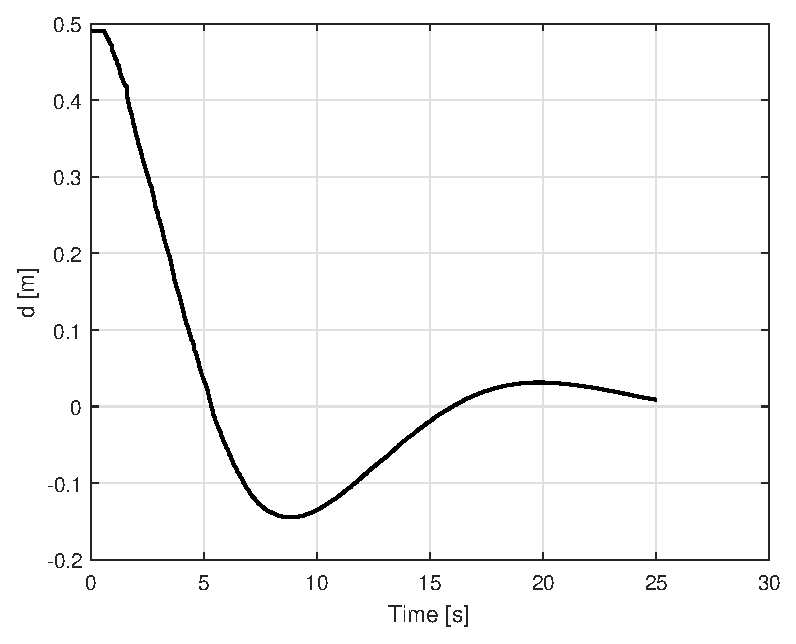
\includegraphics[width=0.36\textwidth]{figs/matlab/lineFollower/error.eps}
    }
    \caption{Performance of MAFOSS in running leader--follower algorithm.}
    \label{fig:performanceLineFollower}
\end{figure}


\subsection{Leader Follower}
The aim of this section is to further evaluate the MAFOSS by running a relatively complex scenario, such as the leader--follower problem, using two EduMOD robots. In this scenario, the leader attempts to follow a circular trajectory and the follower attempts follow behind the leader. The radius of the target circle was set to be $32~[\centi\meter]$, its center was set to $(0,0)~\si{\meter}$, and the desired distance offset between the leader and follower was $15~[\centi\meter].$ The leader was initially placed at $(x,y) = (0.1, -0.2)~\si{\meter}$ with an orientation of $\theta = 0$ while the follower was initially placed at $(x,y) = (-0.2, -0.2)~\si{\meter}$ with an orientation of $\theta = 0$ %% 
\begin{figure}
    \centering
    \subfigure[][]{
    \label{fig:trajectoryLeaderFollowerPic1}
    \includegraphics[width=0.42\textwidth]{figs/img/leaderFollowerAt5.PNG}
    }\\
    \subfigure[][]{
    \label{fig:trajectoryLeaderFollowerPic2}
    \includegraphics[width=0.42\textwidth]{figs/img/leaderFollowerAt60.PNG}
    }    
    %\includegraphics{}
    \caption{MAFOSS running leader--follower algorithm using two eduMOD differential drive mobile robots.}
    \label{fig:trajectoryLeaderFollowerPictures}
\end{figure}
%
follow a leader robot that navigates along a circular path defined by %
%
\begin{subequations}
  \label{eq:refTrajectory}
\begin{align}
  x^{[d]}(t) &= x_c + R\cos(\alpha t)\\
  y^{[d]}(t) &= y_c + R\sin(\alpha t), 
\end{align}  
\end{subequations}

%
where $(x_c,y_c)$ is the coordinate of the center of the circular path with radius $R>0,$ $\alpha$ is the angular rate parameter of the circle at time $t\ge 0.$ The tangent of the trajectory~\eqref{eq:refTrajectory} gives the angle $\theta^{[d]}(t),$ which is computed as $\theta^{[d]}(t) = \mathrm{atan2}(\dot y^{[d]},\dot x^{[d]}).$  The  linear and angular speeds of the leader robot are given by %
%
% \begin{subequations}
\begin{align*}
  \nu^{[d]} = \sqrt{(\dot x^{[d]})^2 + (\dot y^{[d]})^2}~~\text{and}~~
  \omega^{[d]}  = \frac{\ddot y^{[d]} \dot x^{[d]}-\ddot x^{[d]} \dot y^{[d]}}{(\nu^{[d]})^2}.
\end{align*}
% \end{subequations}
%
The follower robot can be  modeled as a unicycle with its kinematics given in~\eqref{eq:unicycleModel}. The problem is to find the linear and angular speeds, $\nu(t)$ and $\omega(t),$ of the follower robot so that it follows the leader robot that follows the reference trajectory~\eqref{eq:refTrajectory} while maintaining a constant geometric distance. %  
%
\begin{figure}
    \centering
    \subfigure[][]{
    \label{fig:trajectoryLeaderFollower}
    \includegraphics[width=0.48\textwidth]{figs/matlab/leaderFollower/trajectory.eps}
    }\\
    \subfigure[][]{
    \label{fig:errorLeaderFollower}
    \includegraphics[width=0.52\textwidth]{figs/matlab/leaderFollower/leaderFollowerImplementDistance.eps}
    }
    \caption{Performance of MAFOSS in running leader--follower algorithm.}
    \label{fig:performanceLeaderFollower}
\end{figure}
%
For the robot to follow the circular path, let us define the position error
%
\begin{align*}
    e(t) = \sqrt{(x^{[d]}(t) - x(t))^2+(y^{[d]}(t) - y(t))^2} - d_{\text{offset}}
\end{align*} 
%
with $d_{\text{offset}}$ being the distance that the robot supposed to maintain from the desired position $(x^{[d]}(t),y^{[d]}(t)).$ The robot's linear speed to follow the path is given by  
%
\begin{align*}
  \nu(t) = K_ve(t) + K_i\int_0^t[e(t)]\mathrm{dt},
\end{align*}
%
where $K_v, K_i>0$ are constant proportional gains. The robot is directed to steer towards the circle with a steering angle given by%
%
%\begin{align*}
  $\gamma = K_\gamma \tilde\theta,$ %
%\end{align*}
%
where $\tilde\theta = (\theta^{'} - \theta)$ with $\theta^{'} = \mathrm{atan2}(y^{[d]}-y,x^{[d]}-x)$ and the proportional gain $K_\gamma>0.$ Note that the angular difference $\tilde\theta\in (-\pi,\pi].$ The values of the parameters used in this experiment are $K_v = 0.35,~K_i = 0$ and $K_\gamma = 0.45.$ The performance of MAFOSS in running a simple leader--follower algorithm is demonstrated in Fig.~\ref{fig:trajectoryLeaderFollowerPictures}, where the follower is following the leader robot on the circular path. The X-Y trajectories of these robots and their distance are shown in Fig.~\ref{fig:performanceLeaderFollower}. As can be seen, the proposed MAFOSS has the ability to run multi-agent algorithms with various complexities. 




\section{Conclusion}
\label{sec:conclusion}
In this paper, we have presented a new framework, MAFOSS, that can be used to implement algorithms for multi-agent systems. Two different experiments have been conducted to show the proposed framework's ability to conduct motion control algorithms using multiple differential drive mobile robots/agents. A potential future work will include testing the proposed MAFOSS for implementing more complex multi-agent control algorithms, such as area coverage control and cooperative estimation while incorporating sensory measurements. 



%%% Local Variables:
%%% mode: latex
%%% TeX-master: "../finalReportMainV1"
%%% End:
